\documentclass[xcolor={usenames,dvipsnames,svgnames,table}, aspectratio=43]{beamer}
\usepackage[utf8x]{inputenc}
\usepackage[T1]{fontenc}
\usepackage{listings}
\usepackage{listingsutf8}				% package PAS PAR DEFAUT + ? \usepackage{textcomp}

\usepackage{verbatim}
\usepackage{tikz}
\usepackage{tkz-graph}

\usepackage{fancybox}
\setbeamercolor{btcolor}{fg=black,bg=gray}
\usepackage{corse-slides}
\usefonttheme[onlymath]{serif}
\renewcommand{\emph}[1]{{\usebeamercolor[fg]{titlelike}#1}}

%symboles, couleurs, algorithmes
\colorlet{green2}{green!50!black}
\newcommand{\before}{\prec_{\mbox{\scriptsize seq}}}
\newcommand{\violet}[1]{{\color{violet}{#1}}}
\newcommand{\red}[1]{{\color{red}{#1}}}
\newcommand{\blue}[1]{{\color{blue}{#1}}}
\newcommand{\green}[1]{{\color{green2}{#1}}}
\newcommand{\gray}[1]{{\color{gray}{#1}}}
\newcommand{\mysmiley}{\Large \color{red}{\smiley}}
\newcommand{\sad}{\includegraphics[width=1em]{fig/flag-smiley-sad.png}}

\usepackage{fancyvrb}
\usepackage{amsmath,txfonts}
\usepackage{color}
\newcommand{\HI}[1]{\textcolor{gray}{#1}}
\newcommand{\var}[1]{$#1$}
\def\lien{$\multimapdotboth$}

\usepackage{ulem}

\lstset{
	tabsize=4,
%	frame=single,
	breaklines=true,
	basicstyle=\ttfamily\tiny,
	frame=tb,
	framerule=0.2pt,
%	frameround={tttt},
	showstringspaces=false,
	language=c,
%	linewidth=0.95\textwidth,
	keywordstyle=\color{black}\bfseries,
%	keywordstyle=\color{blue},
	commentstyle=\color{OliveGreen},
	stringstyle=\color{red}\itshape,
	inputencoding=utf8/latin1,
	numbers=left,
	numberstyle=\tiny,
	numbersep=5pt,
% OMP define
emph={\#,pragma, taskwait, omp, task, depend, affinity, init}, emphstyle=\color{RoyalBlue}\bfseries,
emph={[2]in,inout,out,cw}, emphstyle={[2]\color{BrickRed}\bfseries},
emph={[3]tied,untied,shared}, emphstyle={[3]\color{Gray}\bfseries},
emph={[4]lu0,fwd,bdiv,bmod}, emphstyle={[4]\color{DarkGreen}\bfseries},
emph={[5]cw}, emphstyle={[5]\color{DarkViolet}\bfseries},
}
\setbeamertemplate{itemize item}[circle]
\setbeamertemplate{section in toc}[circle]
\setbeamertemplate{subsection in toc}[square]
%\setbeamercolor{itemize item}{bg=BrickRed, fg=red}
%\setbeamercolor{section number projected}{bg=BrickRed, fg=white}
%\setbeamercolor{subsection number projected}{bg=BrickRed, fg=white}

\beamertemplatenavigationsymbolsempty
\usepackage{appendixnumberbeamer}

\title[Séminaire au vert]{Scheduling Cholesky factorization on NUMA architectures: combining theory and practice}
\author[J. Langou, P. Virouleau]{
Julien Langou, Philippe Virouleau}
%FIXME, ajouter denver correctement
\institute[CORSE/AVALON]{Inria - CORSE/AVALON teams}
\date{January 2nd, 2017}

\begin{document}


\AtBeginSection[]
{
  \begin{frame}
     \frametitle{Outline}
     \tableofcontents[currentsection]
  \end{frame}
}
%\AtBeginSubsection[]
%{
      %\begin{frame}
          %\frametitle{Outline}
              %\tableofcontents[currentsection,currentsubsection]
                %\end{frame}
%}



\section*{Title}
\mymaketitle

\begin{frame}
  \frametitle{Outline}
  \tableofcontents%[pausesections]
\end{frame}


%%%%%
% Avant : Julien
% Après : Philippe
%%%%%

\section{Theory vs practice}

\subsection{Lets compare them!}

\begin{frame}
  \frametitle{What theory can give us}
  \begin{center}
    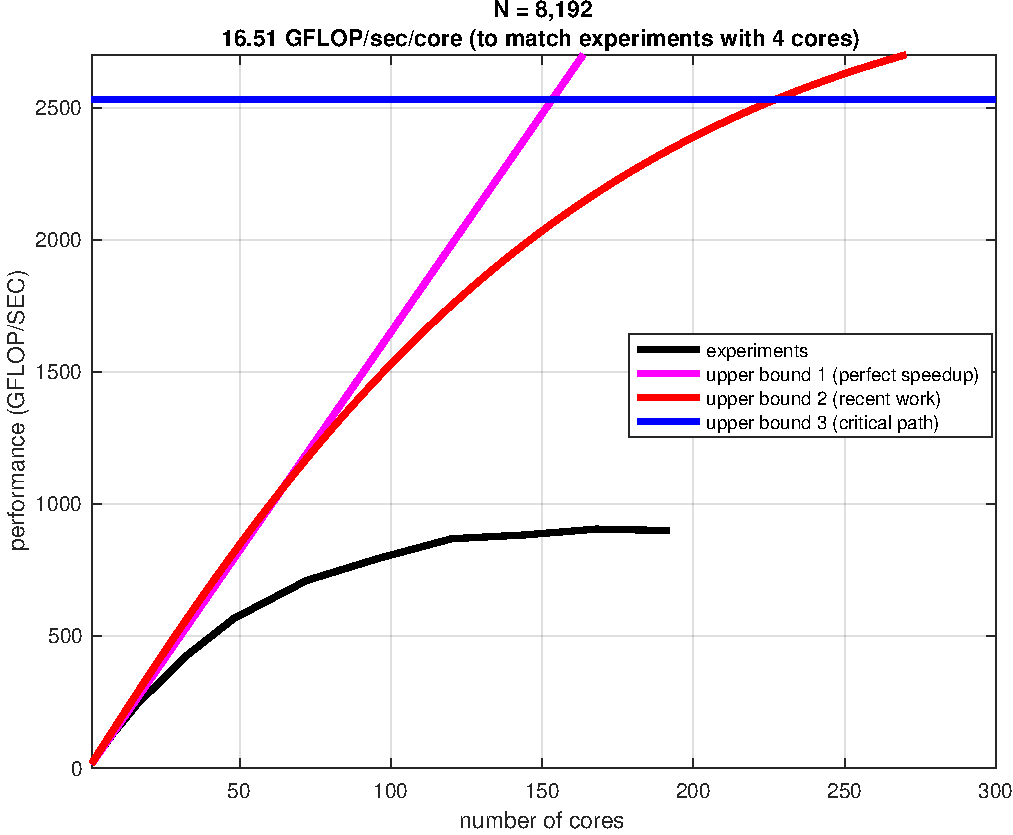
\includegraphics[width=0.7\textwidth]{graph/kaapi_upperbound-crop.pdf}
  \end{center}
\end{frame}

\subsection{What do we run, and on what?}




\begin{frame}[fragile]
\frametitle{Taking a look at the application}


    \begin{lstlisting}

void Cholesky( int N, double A[N][N], size_t NB ) {
#pragma omp parallel
#pragma omp master
  for (size_t k=0; k < N; k += NB) {
#pragma omp task depend(inout: A[k:NB][k:NB])
    clapack_dpotrf(... &A[k*N+k] ...);
                                                                  
    for (size_t m=k+ NB; m < N; m += NB) {
#pragma omp task depend(in: A[k:NB][k:NB]) depend(inout: A[m:NB][k:NB])
      cblas_dtrsm(... &A[k*N+k], &A[m*N+k] ...);
    }
     
    for (size_t m=k+ NB; m < N; m += NB) {
#pragma omp task depend(in: A[m:NB][k:NB]) depend(inout: A[m:NB][m:NB])
     cblas_dsyrk(... &A[m*N+k], &A[m*N+m] ...);

      for (size_t n=k+NB; n < m; n += NB) {
#pragma omp task depend(in:A[m:NB][k:NB], A[n:NB][k:NB]) depend(inout:A[m:NB][n:NB])
        cblas_dgemm(... &A[m*N+k], &A[n*N+k], &A[m*N+n] ...);
      }
    }
  }
}
\end{lstlisting}
\uncover<2>{
\begin{tikzpicture}[overlay, remember picture]
\node[anchor=south east] (img2) at (current page.335) {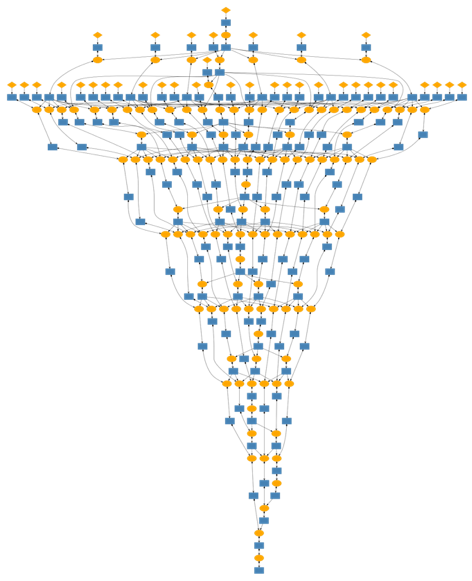
\includegraphics[width=0.4\textwidth]{graph/dfg_depotrf.png}};
    \end{tikzpicture}
}
%Texte : dépendances inter itérations aussi
\end{frame}


\begin{frame}
\frametitle{NUMA architecture overview}
%Texte : dire ce que ça veut dire NUMA, que les données sont partagées, décrire idchire
\begin{columns}[T,onlytextwidth]
  \column{0.42\textwidth}
  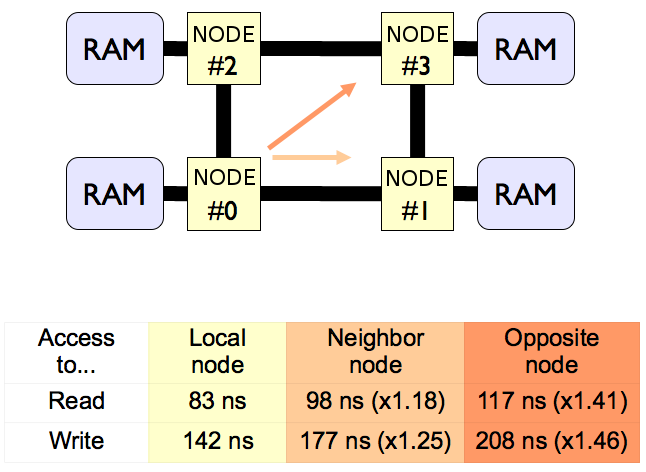
\includegraphics[scale=0.3]{graph/NUMA-latences}
  \column{0.40\textwidth}

  \begin{block}{Description}
    \begin{itemize}
      \item Shared memory
      \item Machine = multiple nodes
      \item Node = multiple cores + a subset of the RAM
    \end{itemize}
  \end{block}

\end{columns}
\begin{alertblock}{Main consequence}
  Task execution time depends on its placement and on its data placement.
\end{alertblock}

\end{frame}

\section{Runtime approaches and extensions}

\subsection{An overview of the problematics}

\begin{frame}[fragile]
\frametitle{Problematics and approaches}
\only<1>{

\begin{block}{The programmer should:}
    \begin{itemize}
      \item be able to give locality hints to the runtime
    \end{itemize}
\end{block}

\begin{block}{The runtime has to:}
    \begin{itemize}
      \item do the load balancing
      \item \alert{be NUMA aware}
        \begin{itemize}
            \item data distribution
            \item data locality
        \end{itemize}
    \end{itemize}
\end{block}


}
\only<2-3> {
  %Texte : deux problèmes majeurs, la distribution des données, la localité des données
\begin{block}{Data distribution}
    \begin{itemize}
      \item Memory divided into multiple nodes
      \item Remote access is expensive !
      \item Needs : control data distribution
    \end{itemize}
\end{block}

\uncover<3>{

  \begin{block}{Standard approaches}
    Using numactl :
    \begin{itemize}
      \item page-level distribution
      \item Data specified in \textit{depend} clauses may use multiple pages!
    \end{itemize}
    Using specific tools and libraries:
    \begin{itemize}
      \item Manual allocation of (huge) arrays
      \item Manual or automatic node selection
    \end{itemize}
  \end{block}

}
}
\only<4-5> {
\begin{block}{Data locality, scheduling}
  Assuming data have been distributed:
    \begin{itemize}
      \item Remote access is expensive (bis)!
      \item One task shall execute close to the data it uses
      \item How to know which data is important?
    \end{itemize}
\end{block}

\uncover<5>{
  \begin{block}{Standard approaches}
    Independent tasks:
    \begin{itemize}
      \item Hierarchical tasks-queues
      \item depth-first execution : cache reuse
    \end{itemize}
  \end{block}

}
}

\end{frame}


\subsection{Extending OpenMP}

\begin{frame}[fragile]
\frametitle{Data distribution}
\begin{columns}[T,onlytextwidth]
  \column{0.45\textwidth}
\begin{block}{'init' clause for parallel regions}
Express how ready tasks should be distributed.

      \textcolor{YellowOrange}{
        In the example: cyclicly distributed over the NUMA nodes.
    }
\end{block}


  \column{0.51\textwidth}

\begin{block}{Example}
  \begin{lstlisting}[numbers=none]
  #pragma omp parallel init(cyclicnuma)
  #pragma omp single
  {
    for (/* all blocks */) {
      #pragma omp task depend(out:block[0:])
      init_block(block);
    }
  }
  \end{lstlisting}
\end{block}
\end{columns}

\end{frame}

\begin{frame}[fragile]
\frametitle{Data locality}
\begin{columns}[T,onlytextwidth]
  \column{0.5\textwidth}
\begin{block}{Affinity clause for tasks}
Express an affinity between a task and "something" on the machine
  \begin{itemize}
    \item Thread

      \textcolor{YellowOrange}{
      This task shall be executed on a place near to this thread
    }
    \item Data

      \textcolor{YellowOrange}{
      This data shall be executed on a place near to this data
    }
  \end{itemize}

\end{block}


  \column{0.45\textwidth}

  \small{Cholesky's snippet:}

\begin{lstlisting}[numbers=none]
/*...*/
for (n = k+1; n < m; n++) {
#pragma omp task depend(in:dA[k][n],
                           dB[k][m])
                 depend(inout:dC[n][m]])
                 affinity(data:dC)
    cblas_dgemm(dA, dB, dC, /*...*/);
}
/*...*/
\end{lstlisting}
\end{columns}

\end{frame}




\subsection{Extending the runtime}

%On a des problèmes, les voila

\begin{frame}[fragile]
\frametitle{Prerequisites}
\begin{block}{Runtime system}
  Uses workstealing, one tasks queue per core, one tasks queue per NUMA node.
    \begin{figure}
        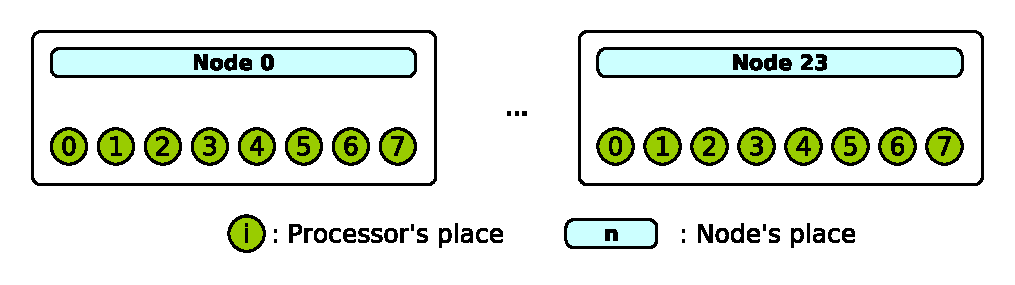
\includegraphics[width=0.8\textwidth]{graph/topology.pdf}
    \end{figure}
\end{block}


\end{frame}


\begin{frame}[fragile]
\frametitle{Concrete course of actions}

\begin{columns}[T,onlytextwidth]
  \column{0.60\textwidth}
  \vspace{2cm}
  \textbf{A two steps plan:}
  \begin{itemize}
    \item \textit{distribute} the data
    \item \textit{execute} the program given this distribution
  \end{itemize}
\uncover<2> {
  \alert{Exploit the workstealing model to do so}
}
  \column{0.4\textwidth}
\uncover<2> {
  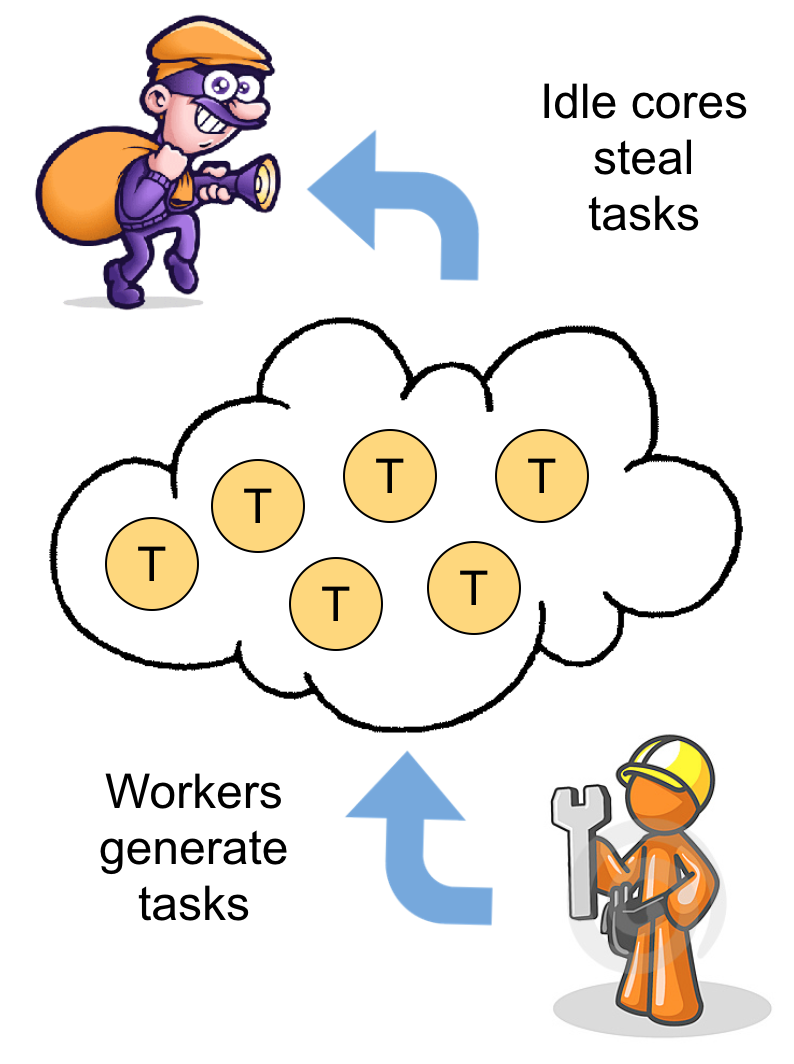
\includegraphics[scale=0.38]{graph/ws}
}
\end{columns}

\end{frame}



%Les algos pour les résoudres, un par un
\begin{frame}[fragile]
  \frametitle{Data distribution}
  \begin{block}{First touch}
    Initialization :
    \begin{itemize}
      \item One parallel region
      \item Independent initialization tasks (data are specified using \verb/depend/ \verb/out/).
    \end{itemize}
  \end{block}
  \begin{block}{+ distributing ready tasks => physical distribution of the data}
    \begin{itemize}
      \item Task distribution over all the nodes/cores
      \item Some strategies example: round-robin, random, ...
    \end{itemize}
  \end{block}
  \alert{Data are distributed}
\end{frame}





\begin{frame}[fragile]
  \frametitle{Data locality and scheduling}

  \begin{block}{Task placement strategies}
    when a task becomes ready, push it to a queue:
    \begin{itemize}
      \item Check hint in \verb/affinity/ clause
      \item Check data in \verb/out/ dependency
      \item Choose relevant queue, e.g: node where the data is physically allocated.
    \end{itemize}
  \end{block}

  \begin{block}{Task selection strategies}
    when a thread becomes idle, chose a queue where to steal from:
    \begin{itemize}
      \item Possible queues : core, node
      \item Several ways of browsing the topology
    \end{itemize}
  \end{block}

\end{frame}

\section{Experimentation results}


\begin{frame}
\frametitle{Applications}

\begin{block}{KASTORS benchmark suite}
  OpenMP 4.0 specific benchmarks

  Kernels used :
  \begin{itemize}
    \item Cholesky (dpotrf)
    \item QR (dgeqrf)
    \item Jacobi
  \end{itemize}

  Cholesky and QR taken from Plasma, modified to use OpenMP (blocked algorithms, using dependent tasks).
  Jacobi is a stencil academic code.
\end{block}

\end{frame}

\begin{frame}
\frametitle{Hardware and software}
\begin{block}{Machine: idchire}
    \begin{itemize}
\item Intel Xeon E5-4640 @ 2.4 GHz, Sandy Bridge
\item 24 NUMA nodes, 8 cores per node, 192 total cores
    \end{itemize}
\end{block}

\begin{block}{Software}
    \begin{itemize}
\item Gcc + libGOMP 6.2
\item Clang + libOMP 3.9
\item OmpSS 16.06
\item Kaapi + extensions

    \end{itemize}
\end{block}
%\begin{figure}
%\begin{center}
%\begin{tikzpicture}[scale=0.6]
%\tikzset{VertexStyle/.append style = {minimum size = 30pt, inner sep = 0pt}}

%\Vertex[x=0, y=0, L=$n_{14,15}$]{n0}
%\Vertex[x=0, y=2, L=$n_{22,23}$]{n4}
%\Vertex[x=0, y=4, L=$n_{8,9}$]{n8}
%\Vertex[x=0, y=6, L=$n_{12,13}$]{n12}
%\Vertex[x=2, y=0, L=$n_{10,11}$]{n1}
%\Vertex[x=2, y=2, L=$n_{6,7}$]{n5}
%\Vertex[x=2, y=4, L=$n_{0,1}$]{n9}
%\Vertex[x=2, y=6, L=$n_{16,17}$]{n13}

%\Vertex[x=4, y=0, L=$n_{20,21}$]{n2}
%\Vertex[x=4, y=2, L=$n_{4,5}$]{n6}
%\Vertex[x=4, y=4, L=$n_{2,3}$]{n10}
%\Vertex[x=4, y=6, L=$n_{10,11}$]{n14}
%\Vertex[x=6, y=0, L=$n_{12,13}$]{n3}
%\Vertex[x=6, y=2, L=$n_{8,9}$]{n7}
%\Vertex[x=6, y=4, L=$n_{18,19}$]{n11}
%\Vertex[x=6, y=6, L=$n_{14,15}$]{n15}

%\Edge(n0)(n5)
%\Edge(n4)(n5)
%\Edge(n1)(n5)

%\Edge(n13)(n9)
%\Edge(n12)(n9)
%\Edge(n8)(n9)

%\Edge(n15)(n10)
%\Edge(n14)(n10)
%\Edge(n11)(n10)

%\Edge(n3)(n6)
%\Edge(n2)(n6)
%\Edge(n7)(n6)

%\Edge(n9)(n5)
%\Edge(n9)(n10)
%\Edge(n5)(n10)
%\Edge(n9)(n6)
%\Edge(n5)(n6)
%\Edge(n10)(n6)

%\end{tikzpicture}
%\end{center}
%\end{figure}
\end{frame}


%\begin{frame}
%\frametitle{Distribution et vol de travail hiérarchique}
%\begin{block}{Distributions}
  %Plusieurs distributions d'initialisation ont été implémentées :
  %\begin{itemize}
    %\item Random -> pousse sur des noeuds NUMA aléatoires
    %\item Cyclic -> round-robin sur tous les coeurs
    %\item Cyclicnuma -> round-robin sur tous les noeud NUMA
  %\end{itemize}

%\end{block}

%\begin{block}{Stratégie de vol hiérarchiques}
  %Plusieurs stratégies de placement et de sélection de tâches :
  %\begin{itemize}
    %\item Placement: pLocNuma (noeud NUMA local), pNumaW (noeud NUMA de la donnée écrite)
    %\item Selection: sRand, sNuma, sProc, sNumaProc (noeud NUMA puis ses coeurs)
  %\end{itemize}
%\end{block}

%\end{frame}



%\begin{frame}
  %\frametitle{Évaluation des stratégies (avec cyclicnuma)}
  %\begin{center}
    %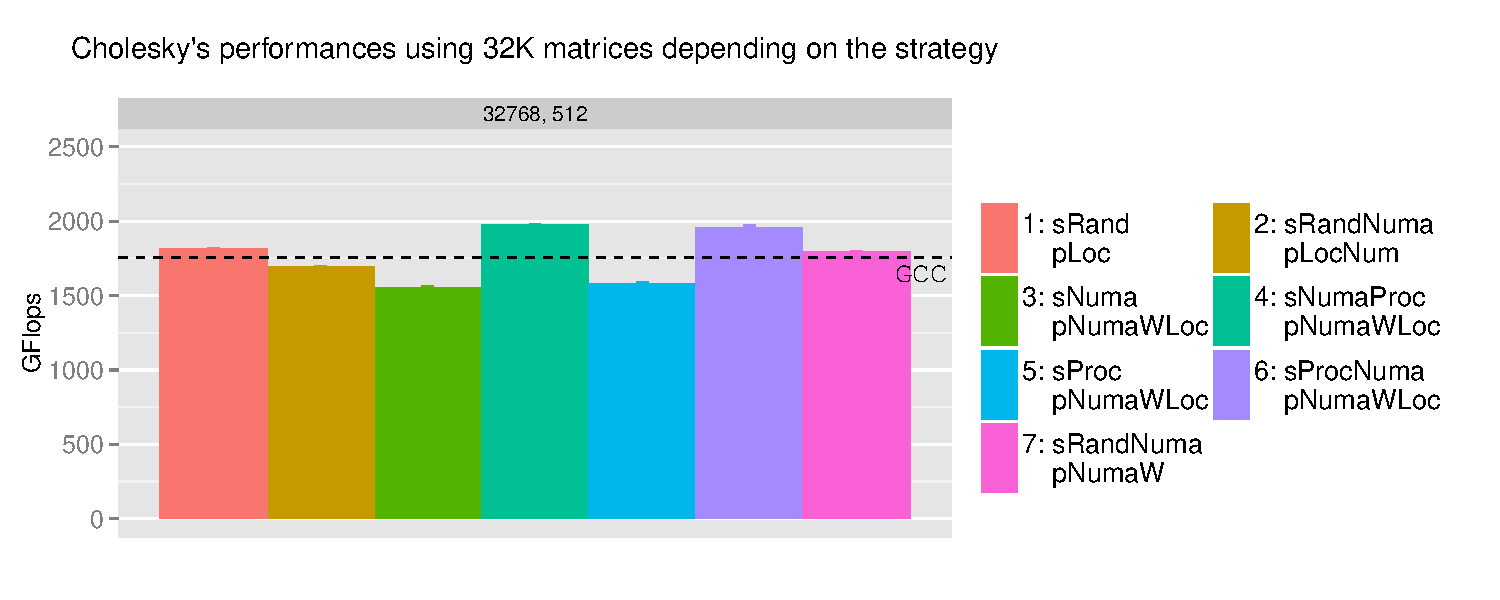
\includegraphics[width=\textwidth]{graph/graph_all_strat.pdf}
  %\end{center}
%\end{frame}

\subsection{Getting there}

\begin{frame}
  \frametitle{Comparison of runtimes on a given problem size}
  \begin{center}
    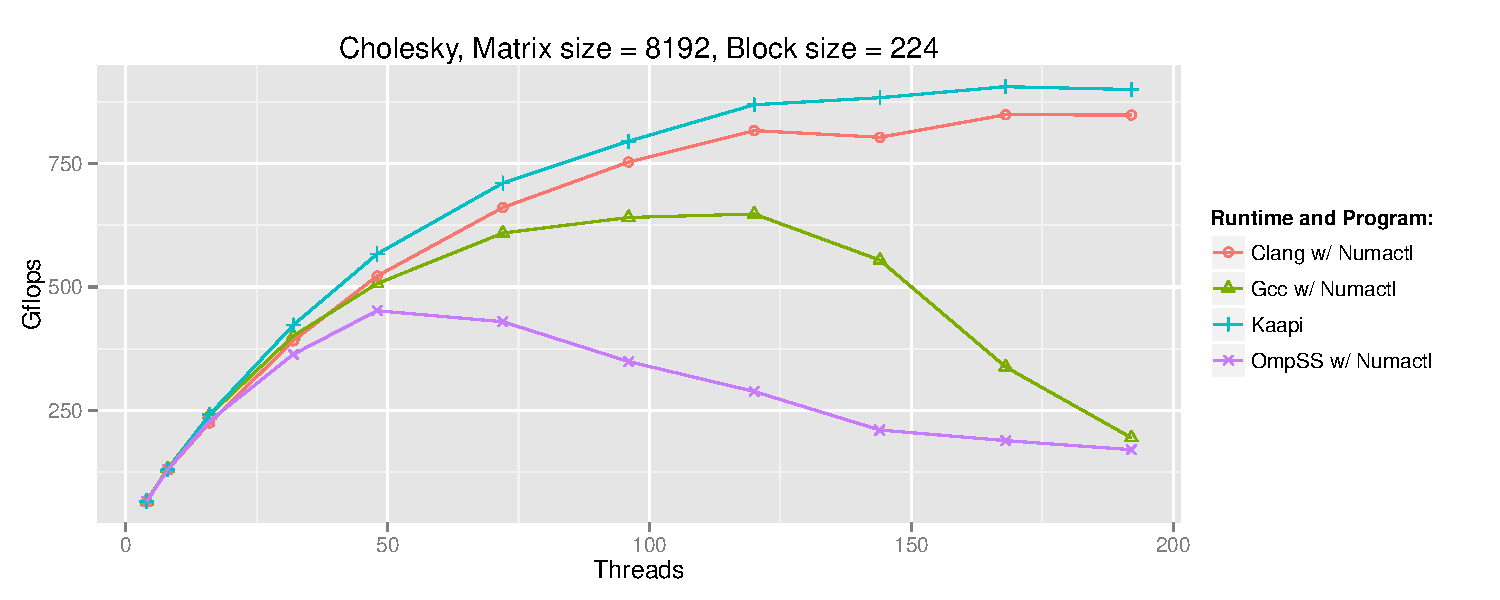
\includegraphics[width=\textwidth]{graph/dpotrf_scale_8k.pdf}
  \end{center}
\end{frame}

\subsection{Explaining the differences, looking for improvements}

\begin{frame}
  \frametitle{Remember...}
  \begin{center}
    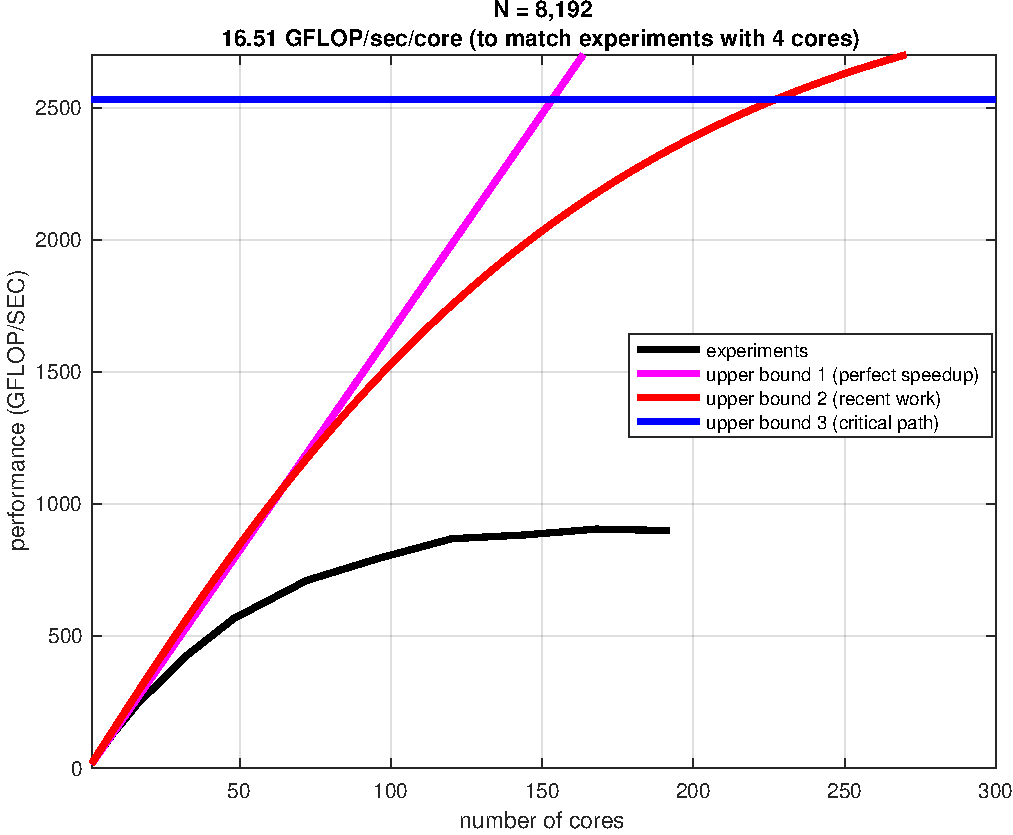
\includegraphics[width=0.7\textwidth]{graph/kaapi_upperbound-crop.pdf}
  \end{center}
\end{frame}

\begin{frame}
  \frametitle{Comparison of work time depending on the task}
  \begin{center}
    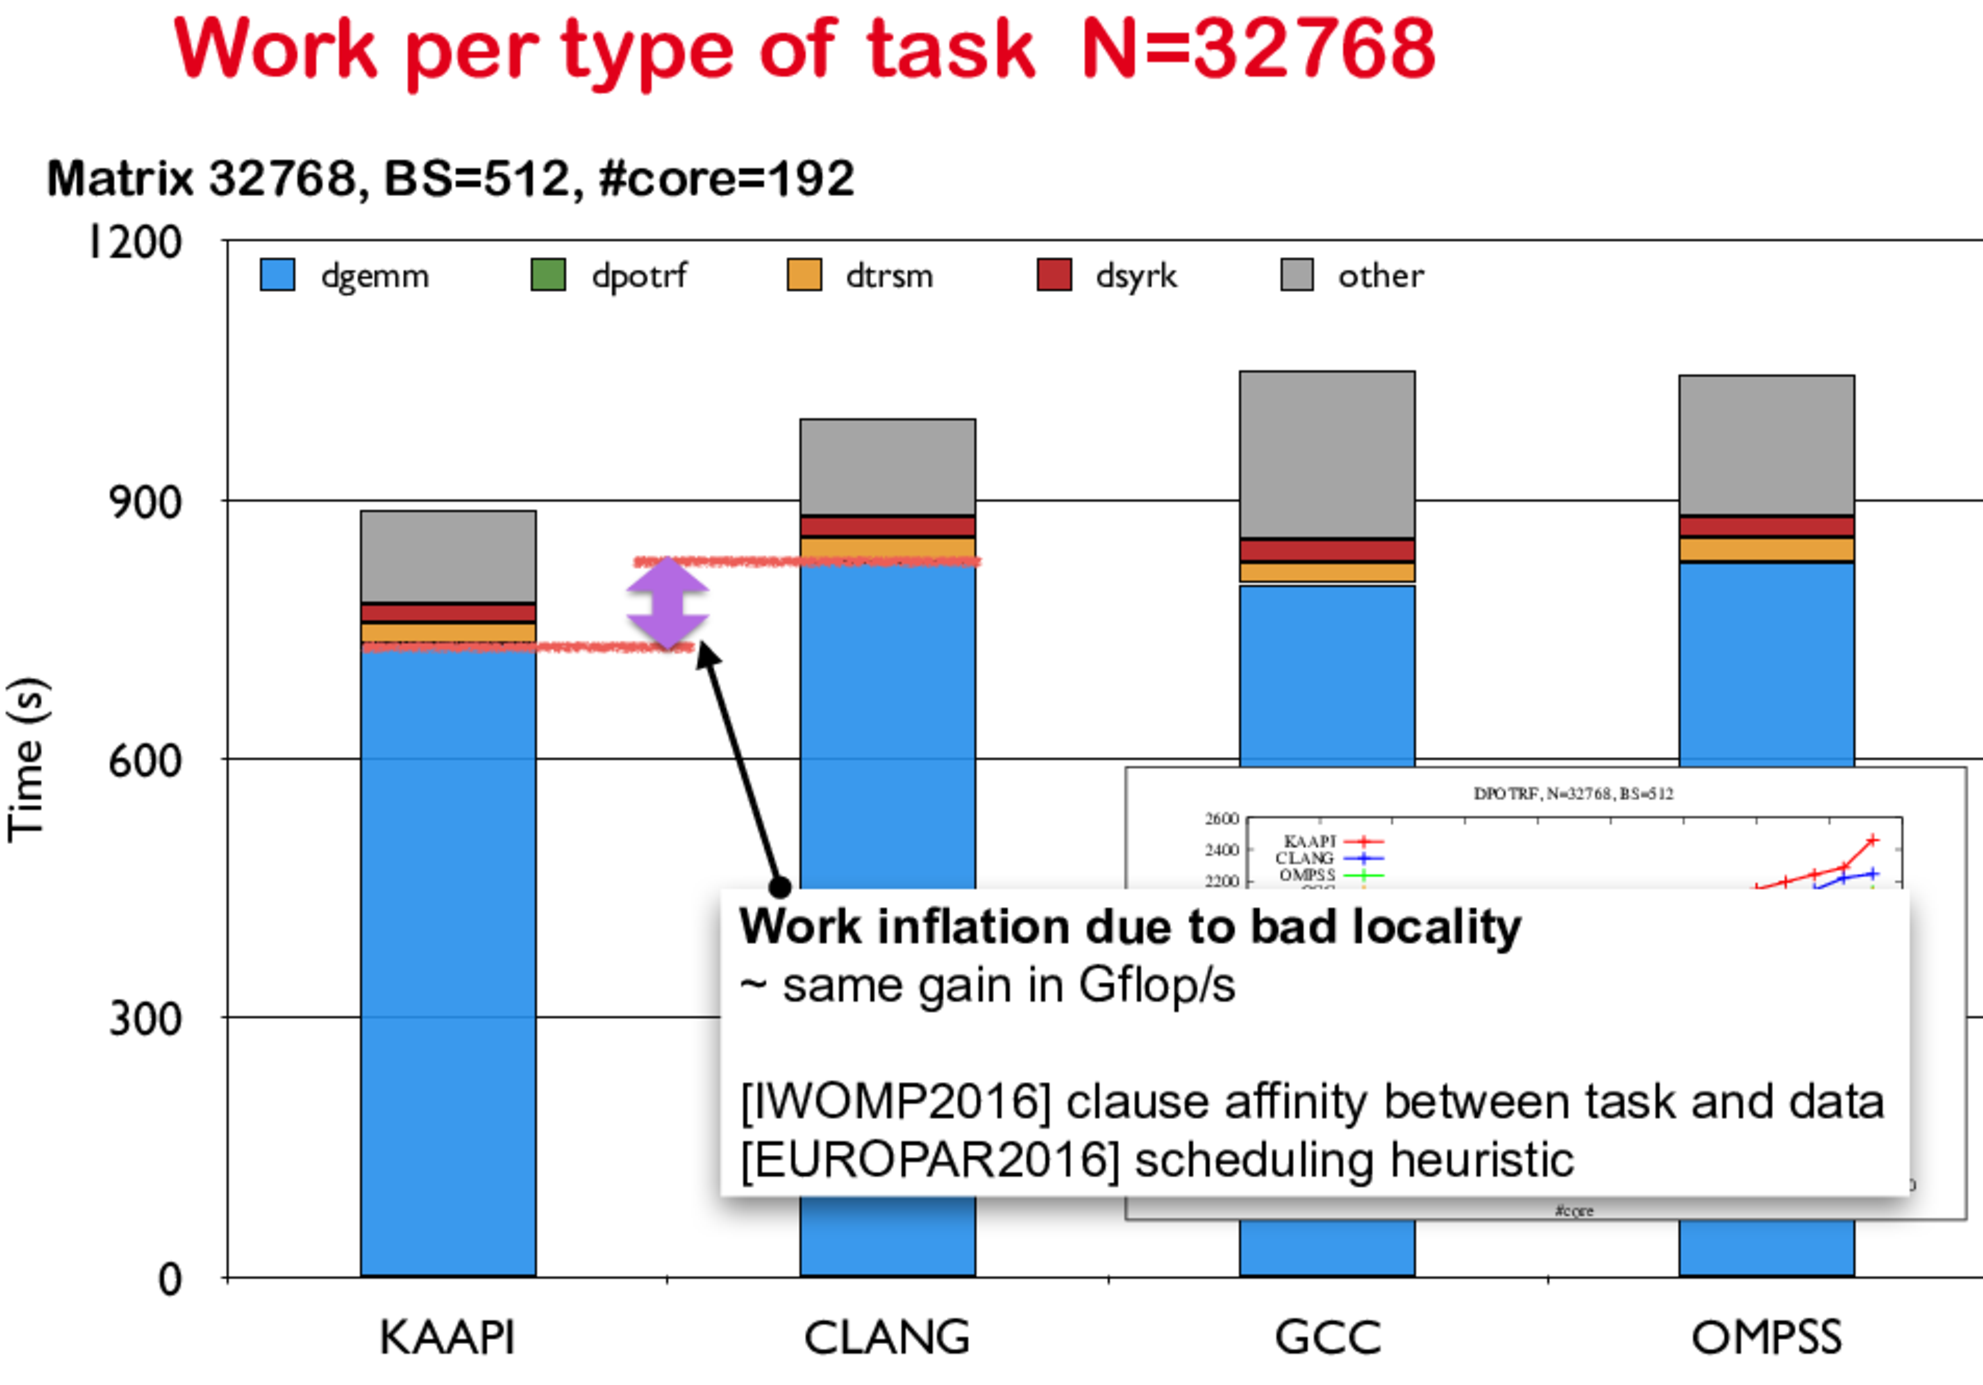
\includegraphics[width=0.85\textwidth]{graph/work_per_task.pdf}
  \end{center}
\end{frame}


\begin{frame}
  \frametitle{A closer look at the average execution time}
  \begin{center}
    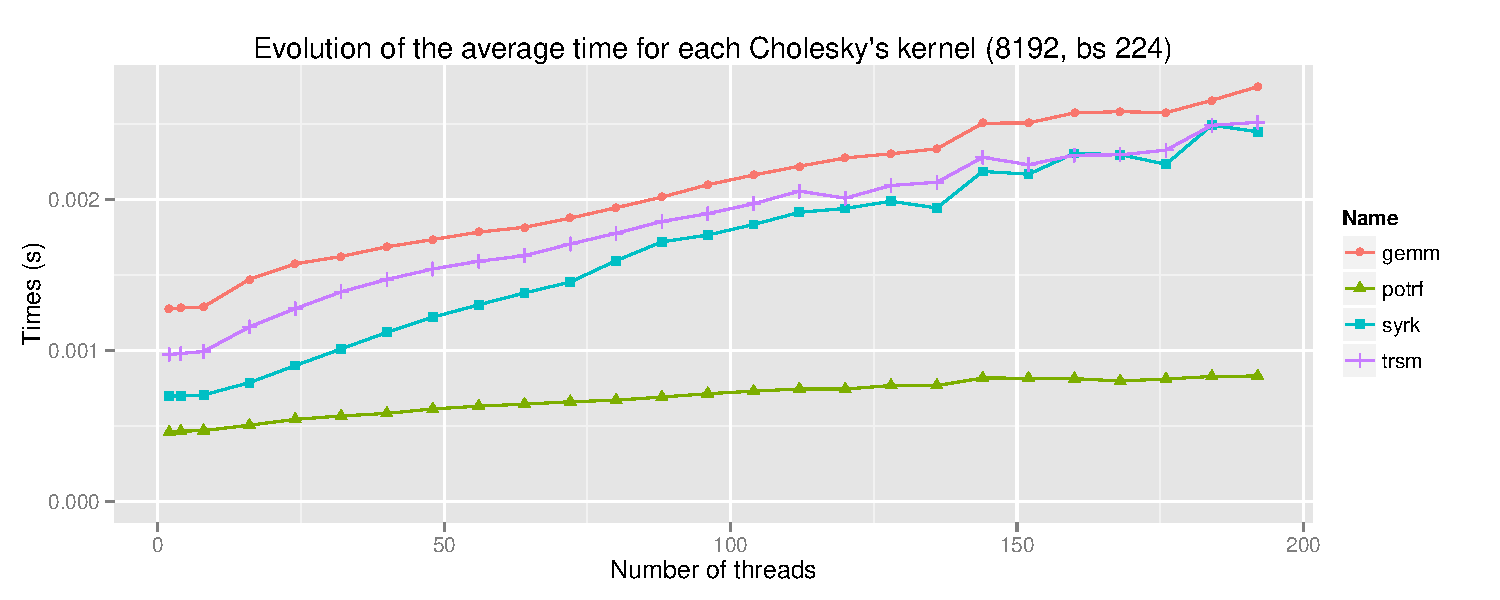
\includegraphics[width=\textwidth]{graph/graph_eval_kernels.pdf}
  \end{center}
\end{frame}

\begin{frame}
  \frametitle{A look at the individual time distribution}
  \begin{center}
    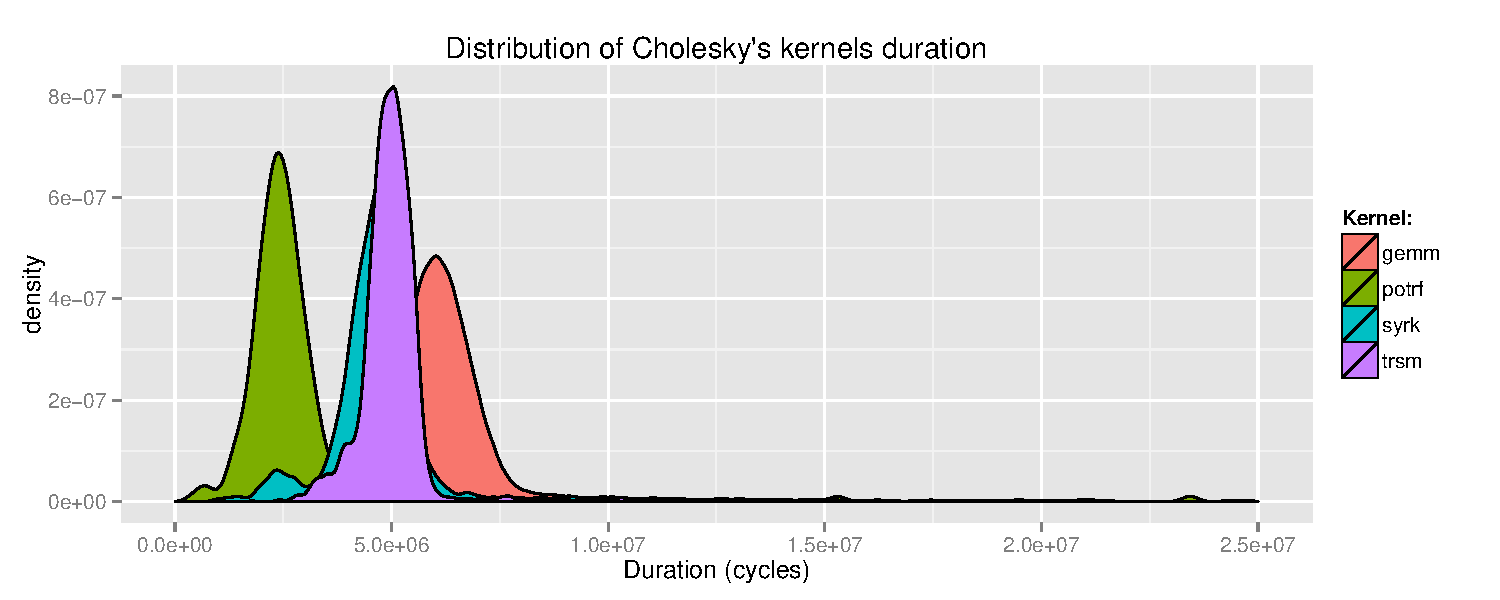
\includegraphics[width=\textwidth]{graph/graph_distrib.pdf}
  \end{center}
\end{frame}

\begin{frame}
  \frametitle{Impact of the NUMA on distribution}
  \begin{center}
    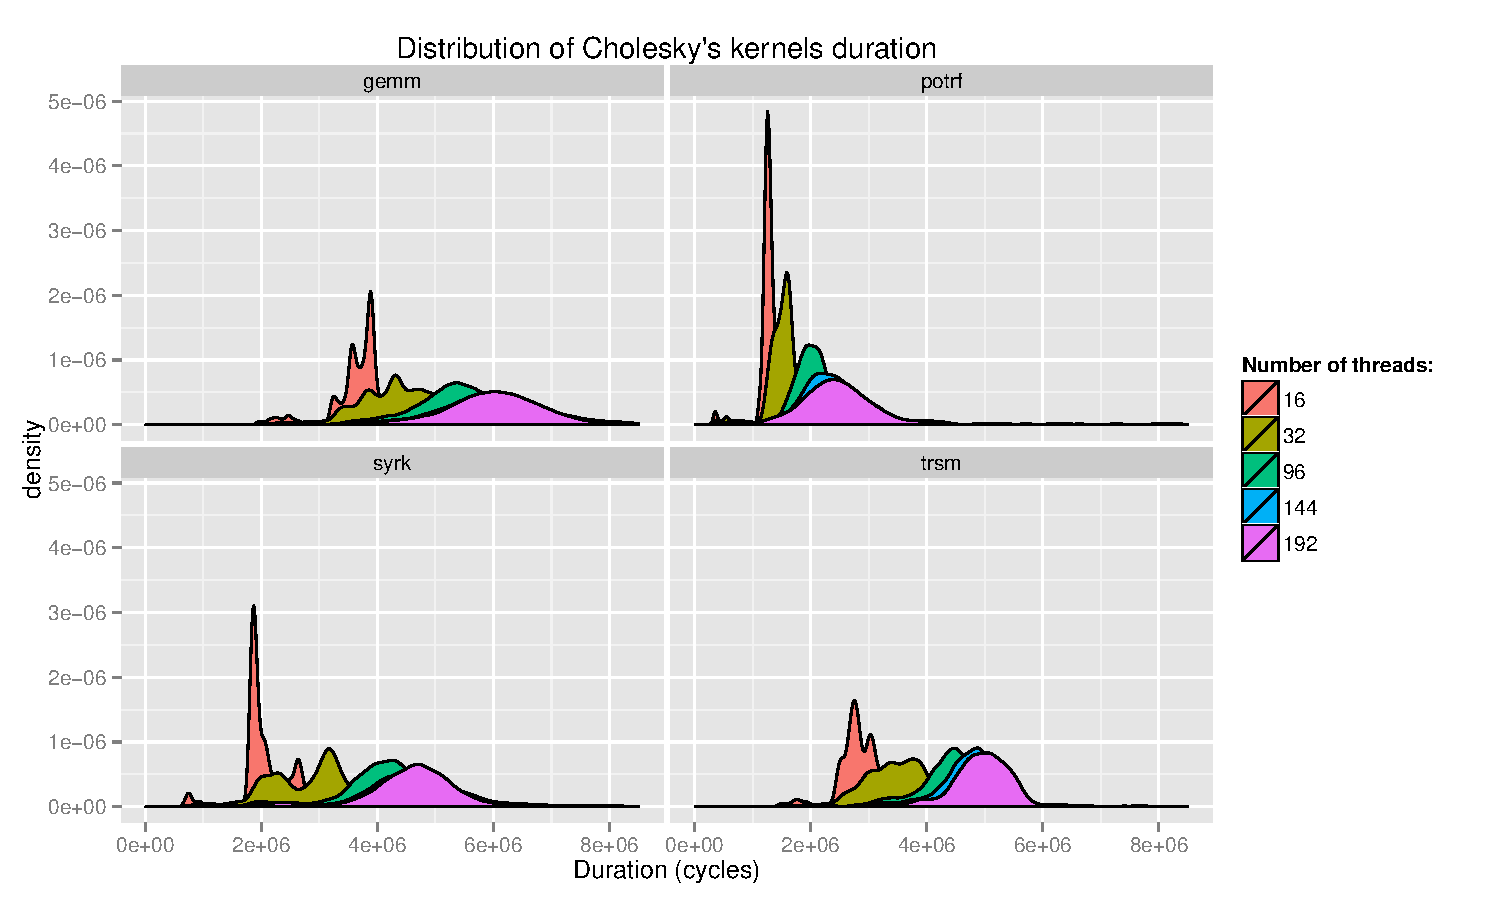
\includegraphics[width=\textwidth]{graph/graph_distrib_overview.pdf}
  \end{center}
\end{frame}




%\begin{frame}
  %\frametitle{Impact of the blocksize}
  %\begin{center}
    %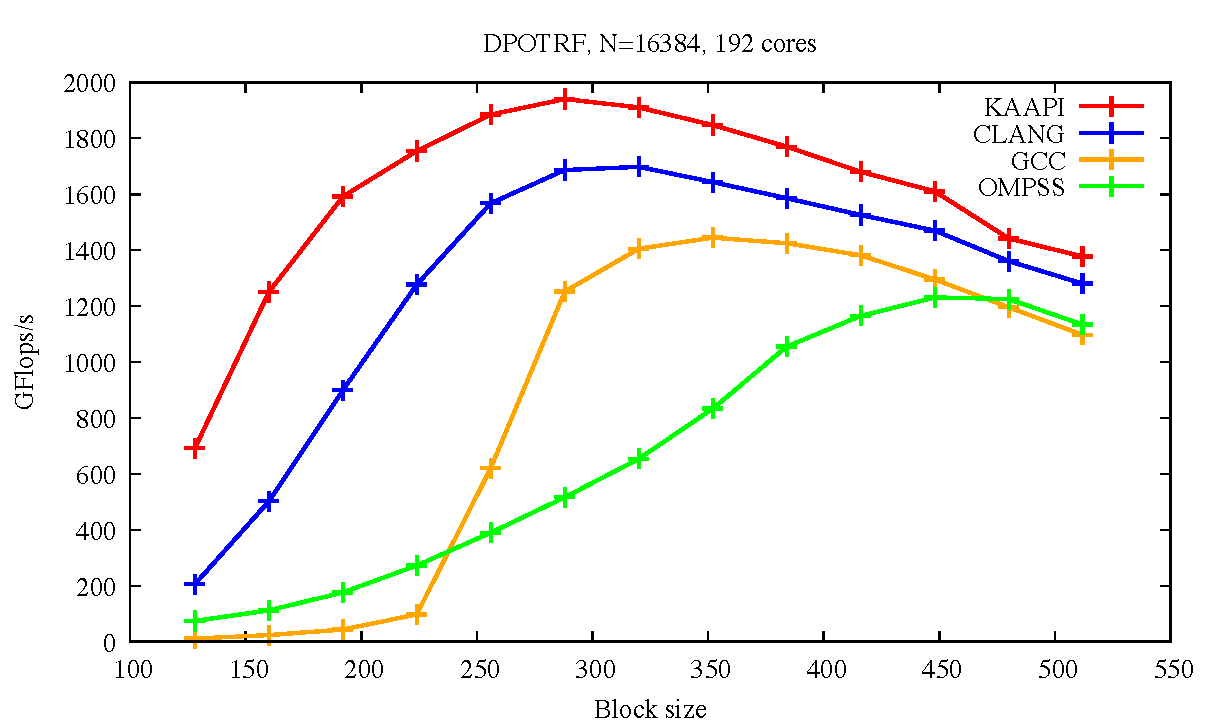
\includegraphics[width=0.85\textwidth]{graph/graph_bs.pdf}
  %\end{center}
%\end{frame}

%\begin{frame}
  %\frametitle{Comparison of runtimes on a small problem size}
  %\begin{center}
    %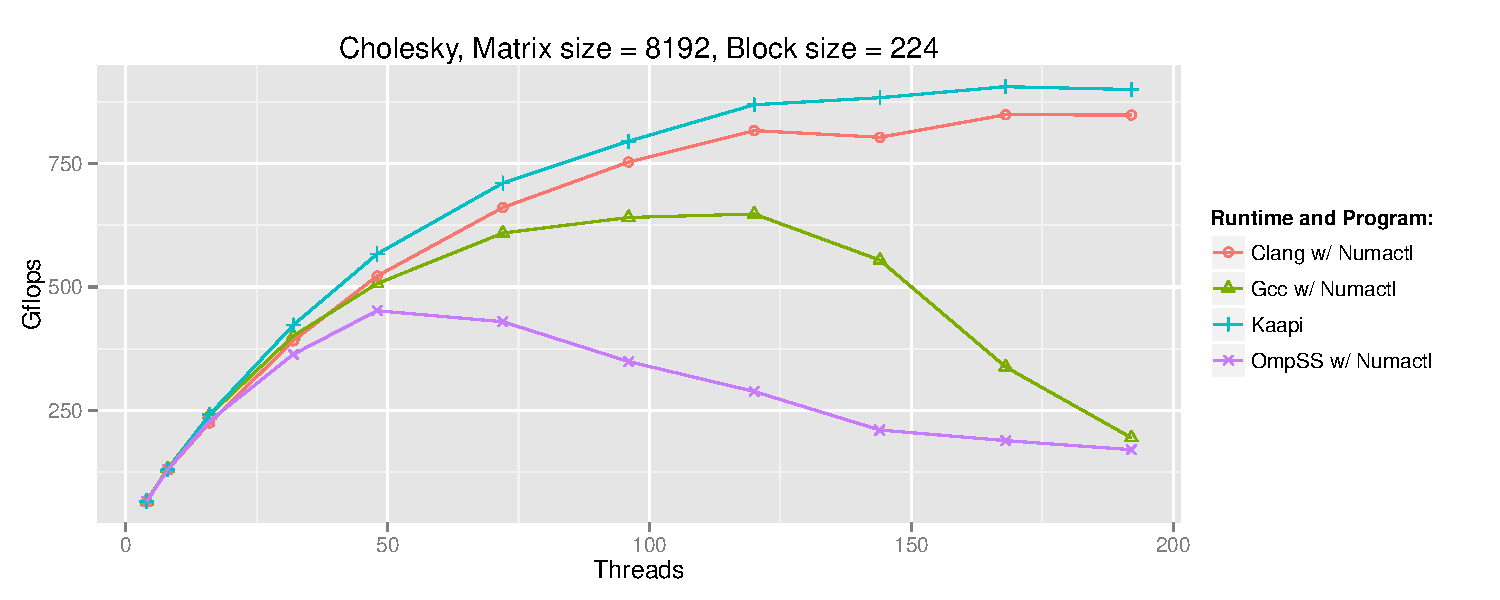
\includegraphics[width=\textwidth]{graph/dpotrf_scale_8k.pdf}
  %\end{center}
%\end{frame}

%\begin{frame}
  %\frametitle{Impact of the strategies using xKaapi}
  %\begin{center}
    %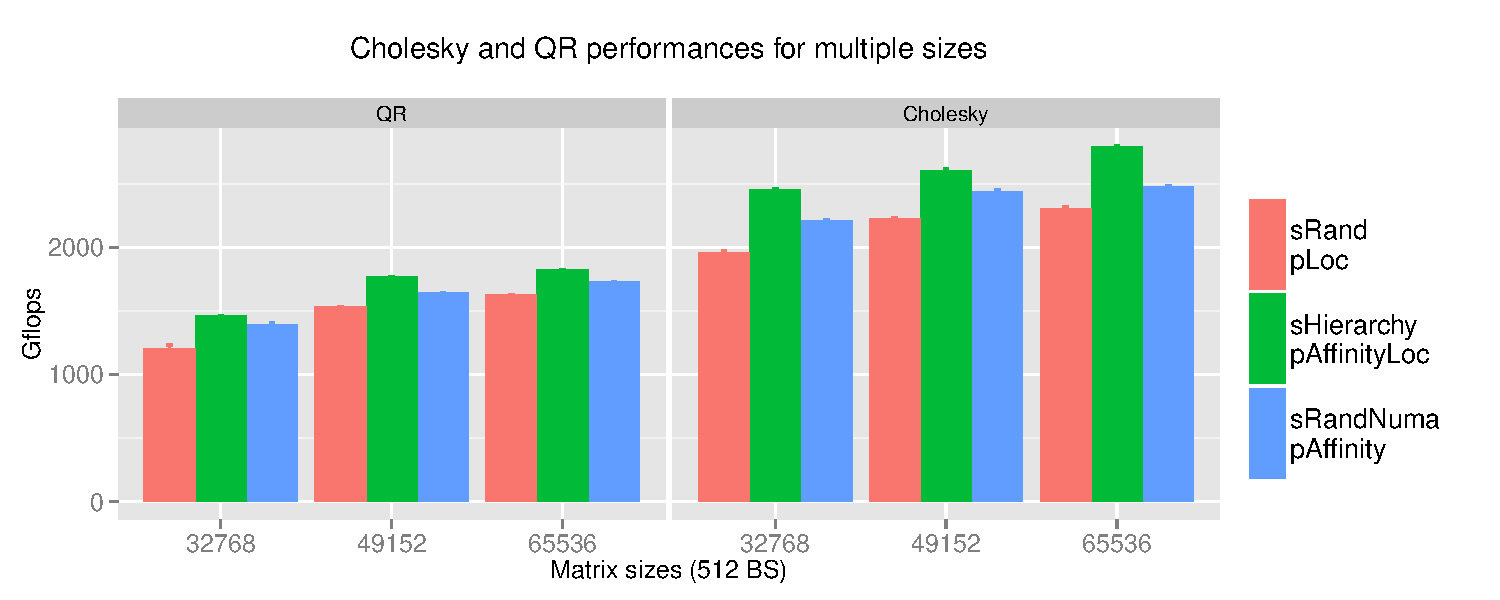
\includegraphics[width=\textwidth]{graph/graph_details_strat.pdf}
  %\end{center}
%\end{frame}


%\begin{frame}
  %\frametitle{Conclusion}
  %\begin{block}{Major impact}
    %Data distribution is the most important factor.
  %\end{block}

  %\begin{block}{How to chose the best strategies combination?}
    %Unfortunately depends on the application...

    %\begin{itemize}
      %\item task + small dataset? -> naive strategies work well
      %\item task + big dataset? -> hierarchical strategies are better
    %\end{itemize}
  %\end{block}
%\end{frame}

\section{Conclusion and future works}



\begin{frame}[fragile]
  \frametitle{Cooperation between the compiler and the runtime}

\begin{block}{All tasks are not similar}
  \begin{itemize}
    \item The compiler can analyse them
    \item The runtime can use this analysis to improve the scheduling
  \end{itemize}
\end{block}

\begin{block}{How to know how our strategies will behave?}
  We somehow need to be able to quickly simulate different strategies, based on the hardware specificities we measure.
\end{block}

\begin{block}{Give it a shot}
  \begin{itemize}
    \item Clang 3.9 fork : https://github.com/viroulep/ + (clang|llvm|openmp)
    \item Kaapi : http://kaapi.gforge.inria.fr/, git branch 'public/xkaapi-3.1'
    \item Kastors : https://gforge.inria.fr/projects/kastors/, git branch 'affinity'
  \end{itemize}
\end{block}

\end{frame}



%\begin{frame}
%\frametitle{Trying the easy way}
%\only<1>{
    %\begin{figure}
        %\includegraphics[width=\textwidth]{graph/graph_defaultmkl.pdf}
    %\end{figure}
    %\vspace{-25pt}
    %\tiny OMP\_NUM\_THREADS=n ./kernel size
%}
%\only<2>{
    %\begin{figure}
        %\includegraphics[width=\textwidth]{graph/graph_defaultmkl_ref.pdf}
    %\end{figure}
    %\vspace{-25pt}
    %\tiny Pic perf in \textcolor{red}{red} !
%}



%\end{frame}
%\begin{frame}
%\frametitle{Common way of dealing with this...}
%\begin{block}{Thread placement}
    %\begin{itemize}
%\item All on same node : reuse cache, nice if compute bound
%\item All distributed accross the machine : average data access faster
%\item Important : no thread migration !
    %\end{itemize}
%\end{block}
%\uncover<2->{
%\begin{block}{Memory distribution}
    %\begin{itemize}
        %\item All memory on the same node : high contention (cf mkl)
        %\item Memory spread accross the node may reduce contention
        %\item Encourage placement of threads near "their" memory
    %\end{itemize}
%\end{block}
%}
%\uncover<3->{
%\begin{block}{Algorithms input}
    %\begin{itemize}
        %\item Choose appropriate size/blocksize for each problem
    %\end{itemize}
%\end{block}
%}
%\end{frame}

%\begin{frame}
%\frametitle{Explicit threads placement and memory distribution}
    %\begin{figure}
        %\includegraphics[width=\textwidth]{graph/graph_16k_mkl.pdf}
    %\end{figure}
    %\vspace{-15pt}
    %\tiny OMP\_NUM\_THREADS=n KMP\_AFFINITY="granularity=fine,explicit,proclist=[...]" numactl -i (...) ./kernel size
%\end{frame}

%\begin{frame}
%\frametitle{Conclusion}
%\begin{alertblock}{Don't}
    %\begin{itemize}
%\item Let the system decide threads placement
    %\end{itemize}
%\end{alertblock}

%\begin{exampleblock}{Do}
    %\begin{itemize}
%\item Pin your threads to avoid migration
%\item Try different threads placement
%\item Control data initialization and distribution
    %\end{itemize}
%\end{exampleblock}

%\end{frame}

%\subsection{Task-based algorithms}
%\begin{frame}[fragile]
%\frametitle{What about task-based OpenMP ?}
    %\begin{lstlisting}

%void Cholesky( int N, double A[N][N], size_t NB ) {
  %for (size_t k=0; k < N; k += NB) {
%#pragma omp task depend(inout: A[k:NB][k:NB]) shared(A)
    %clapack_dpotrf(CblasRowMajor, CblasLower, NB, &A[k*N+k], N );
                                                                  
    %for (size_t m=k+ NB; m < N; m += NB)                          {
%#pragma omp task depend(in: A[k:NB][k:NB]) depend(inout: A[m:NB][k:NB]) shared(A)
      %cblas_dtrsm(CblasRowMajor, CblasLeft, CblasLower, CblasNoTrans, CblasUnit,
                  %NB, NB, 1., &A[k*N+k], N, &A[m*N+k], N );
    %}
     
    %for (size_t m=k+ NB; m < N; m += NB) {
%#pragma omp task depend(in: A[m:NB][k:NB]) depend(inout: A[m:NB][m:NB]) shared(A)
     %cblas_dsyrk(CblasRowMajor, CblasLower, CblasNoTrans,
                 %NB, NB, -1.0, &A[m*N+k], N, 1.0, &A[m*N+m], N );

      %for (size_t n=k+NB; n < m; n += NB) {
%#pragma omp task depend(in:A[m:NB][k:NB], A[n:NB][k:NB]) depend(inout:A[m:NB][n:NB]) shared(A)
        %cblas_dgemm(CblasRowMajor, CblasNoTrans, CblasTrans,
                    %NB, NB, NB, -1.0, &A[m*N+k], N, &A[n*N+k], N, 1.0, &A[m*N+n], N );
      %}
    %}
  %}
%}
%\end{lstlisting}
%\end{frame}

%\begin{frame}
%\frametitle{What about task-based OpenMP ?}
    %\begin{figure}
        %\includegraphics[width=\textwidth]{graph/graph_16k_allruntimes.pdf}
    %\end{figure}
    %\vspace{-15pt}
    %\tiny Using OMP\_PLACES to pin threads
%\end{frame}

%\begin{frame}
%\frametitle{Chosing the right blocksize}
    %\begin{figure}
        %\includegraphics[width=\textwidth]{graph/graph_16k_512_allruntimes.pdf}
    %\end{figure}
%\end{frame}

%\begin{frame}
%\frametitle{Conclusion}
%\begin{exampleblock}{Do}
    %\begin{itemize}
        %\item Give the right amount of work to your runtime
    %\end{itemize}
%\end{exampleblock}
%\begin{block}{Note}
    %\begin{itemize}
        %\item Runtimes should be able to better exploit small blocksizes
    %\end{itemize}
%\end{block}

%\end{frame}

%\begin{frame}
%\frametitle{Even more obvious on 32K matrices !}
%\only<1>{
    %\begin{figure}
        %\includegraphics[width=\textwidth]{graph/graph_32k.pdf}
    %\end{figure}
%}
%\only<2>{
    %\begin{figure}
        %\includegraphics[width=\textwidth]{graph/graph_32k_512.pdf}
    %\end{figure}
%}
%\end{frame}

%\begin{frame}
%\frametitle{Conclusion}
%\begin{block}{Performances don't rely only on runtime}
    %\begin{itemize}
%\item Be aware of grain
%\item Tune your inputs
    %\end{itemize}
%\end{block}
%\begin{block}{Performances aren't *that* bad}
    %\begin{itemize}
%\item Decent scaling up to $\approx$100 cores
%\item Still a big gap to experimental pic perf (dgemm)
    %\end{itemize}
%\end{block}

%\end{frame}

%\subsection{Some more tuning !}
%\begin{frame}
%\frametitle{Tuning threads placement}
%\begin{block}{Threads placement}
    %\begin{figure}
        %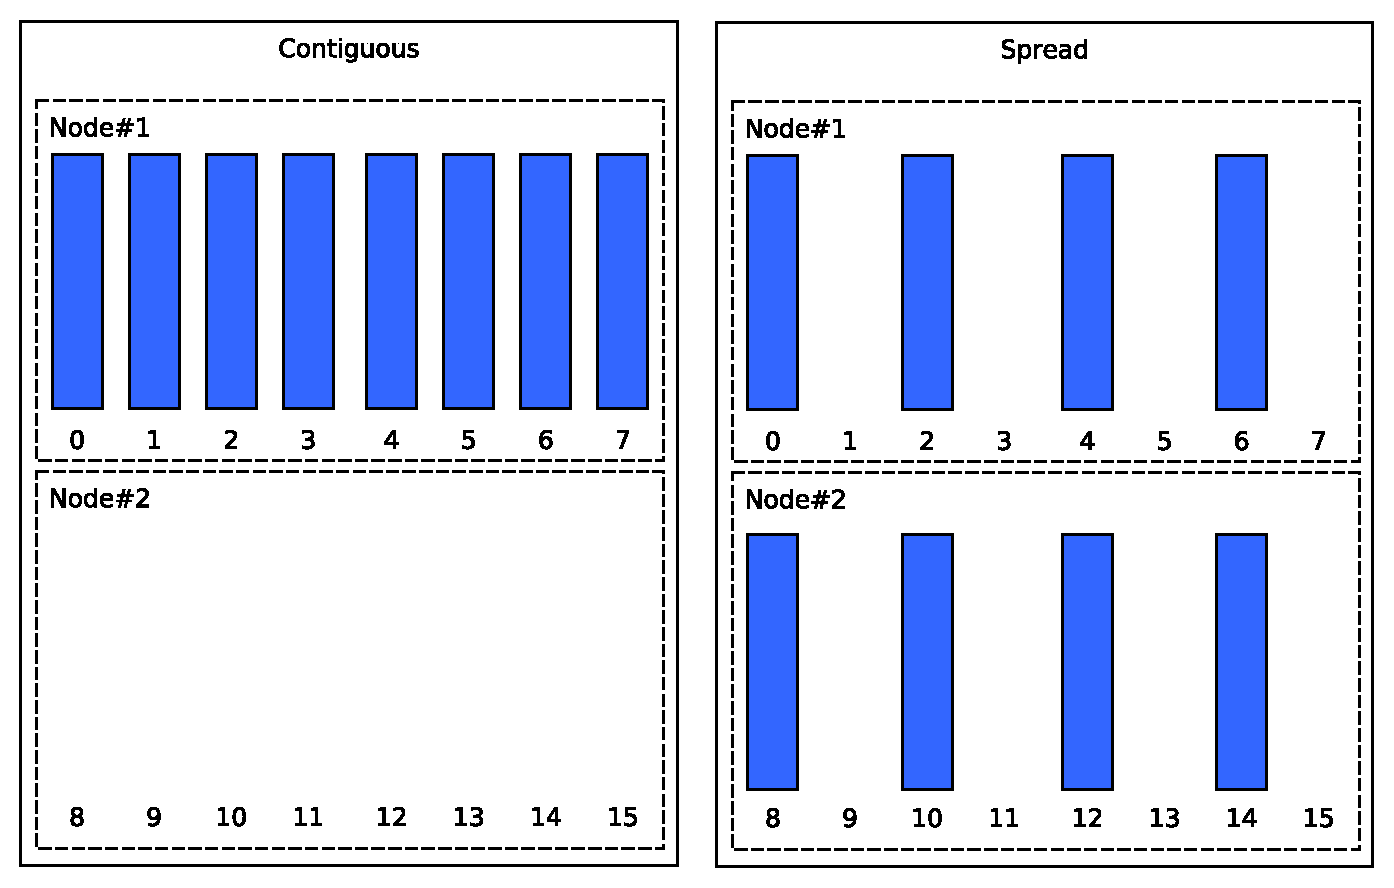
\includegraphics[width=0.8\textwidth]{graph/thread_placement.pdf}
    %\end{figure}
%\end{block}
%\end{frame}


%\begin{frame}[fragile]
%\frametitle{Tuning data distribution}
%\begin{block}{Data initialization}
    %In kastors : initialized accross all the nodes
%\end{block}

%\begin{block}{Distribution at runtime}
    %Using \verb/numactl --interleave=all/
%\end{block}


%\end{frame}

%\begin{frame}
%\frametitle{The big picture...}
    %\begin{figure}
        %\includegraphics[width=\textwidth]{graph/graph_32k_compare_grid.pdf}
    %\end{figure}
%\end{frame}


%\begin{frame}
%\frametitle{Impact of memory distribution + threads placement}
    %\begin{figure}
        %\includegraphics[width=\textwidth]{graph/graph_32k_compare.pdf}
    %\end{figure}
%\end{frame}

%\begin{frame}
%\frametitle{Conclusion}
%\begin{block}{Memory distribution}
    %Actually worst : data is already distributed during initialization
%\end{block}
%\begin{block}{Threads placement}
    %\begin{itemize}
        %\item Not much difference for low and high number of threads
        %\item Nice gain from spreading the threads otherwise
    %\end{itemize}
%\end{block}
%\end{frame}

%\begin{frame}
    %\frametitle{Pic perf summary}
    %\begin{figure}
        %\includegraphics[width=\textwidth]{graph/graph_32k_picperf.pdf}
    %\end{figure}
%\end{frame}
%\begin{frame}
%\frametitle{Overall conclusion}
%\begin{block}{Tuning matters}
    %\begin{itemize}
        %\item Find the right threads placement
        %\item Adapt memory distribution
        %\item Adapt the grain of your application
    %\end{itemize}
%\end{block}
%\end{frame}


%\section{Solving the scalability issue}

%\begin{frame}
%\frametitle{Still some performances to gain}
%\begin{block}{Next step ?}
    %\begin{itemize}
    %\item Improve the algorithm -> cf litterature
        %\item Tune the program to a specific architecture -> not portable
        %\item Improve the runtime/programming model
    %\end{itemize}
%\end{block}
%\end{frame}

%\begin{frame}
%\frametitle{Still some performances to gain}
%\begin{block}{Improving the programming model}
    %\begin{itemize}
    %\item Better architecture aware directives/clauses
        %\item More tools
    %\end{itemize}
%\end{block}
%\begin{block}{Improving the runtime}
    %\begin{itemize}
        %\item Better mapping of data+threads (needs information)
        %\item NUMA aware algorithm (task queue, barrier, etc)
    %\end{itemize}
%\end{block}
%\begin{block}{Ask for compiler help}
    %\begin{itemize}
        %\item Can help automatically detect dependencies, data placement, etc)
    %\end{itemize}
%\end{block}
%\end{frame}

%\begin{frame}[fragile]
    %\frametitle{Conclusion - Current Kaapi state}
%\begin{onlyenv}<1>%
    %Affinity extension, via OpenMP API
    %\begin{lstlisting}
    %[...]
%omp_set_task_affinity( CYCLIC(m,n,6,4), 1 );
%#pragma omp task depend(out:dA[0:ldam*tempnn])
%CORE_dplgsy( bump, tempmm, tempnn, dA, ldam, A.m, m*A.mb, n*A.nb, seed );
    %[...]
%\end{lstlisting}
%Using Klang-omp :
    %\begin{lstlisting}
    %[...]
%#pragma omp task depend(out:dA[0:ldam*tempnn]) affinity( CYCLIC(m,n,6,4) )
%CORE_dplgsy( bump, tempmm, tempnn, dA, ldam, A.m, m*A.mb, n*A.nb, seed );
    %[...]
%\end{lstlisting}
%\end{onlyenv}
%\only<2>{
    %\begin{figure}
        %\includegraphics[width=\textwidth]{graph/graph_32k_512_kaapi.pdf}
    %\end{figure}
%}
%\footnotesize Reminder : target architecture has 24 (4*6) NUMA nodes.
%\end{frame}

%\begin{frame}
    %\frametitle{Fin}
    %\begin{center}
    %Fin
    %\end{center}
%\end{frame}


%\appendix

%\begin{frame}
%\frametitle{Other ongoing works}
%\begin{block}{Using OMPT}
    %\begin{itemize}
%\item IOMP + HPCToolkit
%\item OMPT can be used to gather information about where a thread fetch its data from.

%\item We want a per-task view
    %\end{itemize}

%\end{block}
%\end{frame}

%\begin{frame}
    %\frametitle{Another threads placement (round robin)}
    %\begin{figure}
        %\includegraphics[width=\textwidth]{graph/graph_32k_compare_spreadnode.pdf}
    %\end{figure}
%\end{frame}


\end{document}
